% This is samplepaper.tex, a sample chapter demonstrating the
% LLNCS macro package for Springer Computer Science proceedings;
% Version 2.20 of 2017/10/04
%
\documentclass[runningheads]{llncs}
%

\makeatletter
\@ifclasswith{llncs}{peerreview}{
	\author{}
	\typeout{PEERREVIEW}
	\newcommand\MYhyperrefoptions{
		pdftitle={MessageVortex Protocol -- Sending Messages Anonymously},
		pdfsubject={MessageVortex Protocol},
		pdfkeywords={Messages, Unobservable, Anonymity, Unlinkability, Pseudonymity }
	}
}{
	\typeout{PUBLIC}
	\author{M. Gwerder\inst{1,2}\orcidID{0000-0003-0296-5079}}
	%
	\authorrunning{M. Gwerder}
	\institute{University of Basel, Switzerland \and
		University of Applied Sciences of Northwestern of Switzerland\\
		\email{martin.gwerder@fhnw.ch}\\
		%\url{https://www.fhnw.ch/en/about-fhnw/schools/school-of-engineering/institutes/institute-of-mobile-and-distributed-systems} 
	}
	\newcommand\MYhyperrefoptions{
		pdftitle={MessageVortex Protocol -- Sending Messages Anonymously},
		pdfsubject={MessageVortex Protocol},
		pdfkeywords={Messages, Unobservable, Anonymity, Unlinkability, Pseudonymity }
		pdfauthor={Martin Gwerder},%<!CHANGE
	}
}
\makeatother
\usepackage{xcolor}
\usepackage[\MYhyperrefoptions,pdftex]{hyperref}
\usepackage{graphicx}
\usepackage{appendix}

\usepackage[cmex10]{amsmath}
\DeclareMathOperator{\prng}{prng}
\DeclareMathOperator{\len}{len}
\DeclareMathOperator{\splitPayload}{splitPayload}
\DeclareMathOperator{\mergePayload}{mergePayload}
\DeclareMathOperator{\startsWith}{startsWith}
\DeclareMathOperator{\lendsWith}{endsWith}
\DeclareMathOperator{\addRedundancy}{addRedundancy}
\DeclareMathOperator{\removeRedundancy}{removeRedundancy}
\DeclareMathOperator{\encrypt}{encrypt}
\DeclareMathOperator{\decrypt}{decrypt}

\usepackage[pdftex]{thumbpdf}

\hyphenation{op-tical net-works semi-conduc-tor}

% Used for displaying a sample figure. If possible, figure files should
% be included in EPS format.
%
% If you use the hyperref package, please uncomment the following line
% to display URLs in blue roman font according to Springer's eBook style:
\renewcommand\UrlFont{\color{blue}\rmfamily}
\begin{document}
%
\title{MessageVortex Protocol -- Sending Messages Anonymously}
%
\titlerunning{MessageVortex Protocol}
% If the paper title is too long for the running head, you can set
% an abbreviated paper title here
%
% First names are abbreviated in the running head.
% If there are more than two authors, 'et al.' is used.
%

%
\maketitle              % typeset the header of the contribution
%
\begin{abstract}
In this paper, we introduce an unobservable message anonymization protocol, named MessageVortex. It is based on the zero-trust and peer-to-peer (P2P) principle, and avoids central aspects such as fixed infrastructures within a global network. It scores over existing work by blending its traffic into suitable existing transport protocols, thus making it next to impossible to block it without significantly affecting regular users of the transport medium. It furthermore requires no protocol-specific infrastructure in public networks and allows a sender to control all aspects of a message such as the degree of anonymity, timing, and redundancy of the message transport without disclosing any of these details to the routing or transporting nodes.

\keywords{Messages \and Unobservable \and Anonymity \and Unlinkability \and Pseudonymity }
\end{abstract}
%
%
%
\section{Introduction}
Since whistleblower Edward Snowden disclosed documents, it seems generally accepted that global monitoring of Internet traffic is conducted. According to these documents (verified by \href{http://www.nrc.nl/nieuws/2013/11/23/nederland-sinds-1946-doelwit-van-nsa}{NRC}), NSA infiltrated more than 50k computers with malware to collect classified or personal information. They furthermore infiltrated telecom operators such as Belgacom to collect data and targeted high members of governments even in associated states. 

A message sent throughout the Internet must, even when perfectly encrypted, disclose at least the recipient to the router transporting a message. The sender can be identified by the return path or is identifiable by following the source of packets. Meta information is valuable because frequency and message size disclose important facts about the association and intensity of the relationship of involved parties. %Typical attacks are traffic capturing by network observation or by inserting one or more malicious nodes into a routing network. 

This paper addresses the above-mentioned problems of traffic monitoring by introducing a new  protocol called MessageVortex. Within MessageVortex we consider the whole network as untrusted with the exception of the sending and receiving node. MessageVortex does not leak routing information as only the immediate peers are known to a node. The protocol is able to sustain anonymity\cite{anon_terminology} even under harsh assumptions such as an adversary possessing huge but limited funding, unlimited monitoring capability on the network and a considerable number of own nodes. For a more precise adversary model, see Appendix~\ref{sec:adversary}.

Numerous attempts such as in \cite{minion-design,babel,mixmaster-spec,tor-design,freehaven-berk,herbivore:tr} have been made to anonymize message flow. However, most of them have problems as they rely at least on the partial trust in the nodes routing the messages, or some central infrastructures \cite{hs-attack06,esorics13-cellflood,esorics12-torscan,oakland2013-trawling}. Exit and entry points are important as they may leak information which is otherwise well hidden within the network. By degrading the network, message flows can be redirected and information extracted from the new flows. Additionally, a dedicated transport protocol is easy to block since their implementation can be easily identified by used ports or some protocol properties. Furthermore, most approaches require infrastructure with fixed addressing within the internet, rendering owners vulnerable.

All papers analyzed for this work introduced a new transport layer solving these problems. Only TOR defined an additional transporting mechanism which may be used as an alternate transport medium between two defined nodes to avoid detection. In our approach, we decouple the routing layer from the transport layer completely. By doing so, we introduce new degrees of complexity to attack scenarios, as messages may use any common transport protocol of the used network. 

Our work consists of a routing layer which is completely P2P based without any central protocol specific infrastructure. Any node is a routing node and may be an endpoint. There is no implicit or explicit trust in any particular system of the  network. The original sender of a message controls decoy traffic generation. Even a node generating decoy traffic is unable to differentiate between message and decoy traffic as a Solomon-Reed algorithm is used to blow the message up by adding redundancy information. This redundancy information may be decoy traffic or later required to rebuild data blocks. The redundant blocks are always encrypted, and a multitude of the ciphers block size as they are padded before splitting. This padding before doing the Reed-Solomon operation eliminates the need for padding at the encryption at the block level. This fact makes it very hard to apply brute force to decrypt the content as the padding gives almost no hints whether decryption has been successful or not.

As transport media, we use standard, well known store-and-forward-based protocols. By doing so, the routing logic has no affiliation to the transport layer. Any free-mailer email address or chat account may be converted into a transport media for our protocol without any modification required on the server side. This makes the network very agile on one side at the cost of reliability, as nodes may suddenly appear or disappear. To counter this phenomenon, we may introduce a high degree of redundancy if required and wished by the routing block builder.

Using the MessageVortex protocol, any device with latent or permanent connectivity to the Internet may act as a routing node. 

By applying the zero-trust model, we give full control of all traffic to the original sender of the message. He controls message flow, redundancy, the degree of anonymity, timing, and many more aspects of the message transport throughout the whole network. This is done without disclosing any of these parameters to the participating nodes as they are encoded in the operations and only visible to the node executing them. The operations itself are chosen in such a way that they do not reveal the nature of the traffic.

To limit possibilities of denial-of-service (DoS) within the system and guarantee efficient handling of messages, MessageVortex nodes (in short ``node'') rely on unlinked, ephemeral identities which are created in a proof of work system (PoW). While it is technically easy to use a node, it is hard to carry out traditional attacks against them as all transactions have to be pre-authenticated with PoW puzzles. The amount of work required to disrupt services or conduct traditional attacks against the system grows significantly due to the nonlinear growth of calculation power required when maintaining more ephemeral identities. It is, however, still possible to exhaust external resources such as network bandwidth.\par\nopagebreak
%\ifCLASSOPTIONpeerreview
%\else
%\hfill gwm\par\nopagebreak
%\hfill Mai 27, 2015
%\fi
\subsection{Previous Work}
Generally, not many technologies are used to achieve anonymity or unlinkability as defined in \cite{anon_terminology}. Most analyzed protocols use relays\cite{CHAUM1}, mixes\cite{CHAUM1}, or Dining-Cryptographers-related-networks\cite{chaum-dc} or their variants to achieve anonymization. Numerous protocols have evolved from these technologies:
\begin{itemize}
	\item \emph{TOR}\cite{tor-design}: Mixer-based infrastructure for tunneling TCP-based protocol streams. TOR is a synchronous or near synchronous routing system. The anonymization is based on mixing by using a statical path consisting of an entry node, an exit node, and at least three more intermediate nodes.
	\item \emph{Mixmaster}\cite{mixmaster-spec}: A type-II remailer where all mixes may choose the path on their own logic.
	\item \emph{Babel}\cite{babel}: Mixer-based remailer where the sender chooses the path and sends an onionised message.
	\item \emph{Mixminion}\cite{minion-design}: A type-III remailer offering sender anonymity. Unlike their predecessors, it is no longer based on the SMTP transport protocol. This system requires at least a centralized directory infrastructure.
	\item \emph{Freehaven}\cite{freehaven-berk}: A distributed storage system. The system offers anonymous document storage. To receive a document, a hash of a public key used to sign the document must be known. Known documents may be identified, even if no key is known, and owners of infrastructure might be held responsible if hosting such well-known documents when not confomant to the local jursidictional zone.
	\item \emph{Freenet}\cite{freenet}: Freenet is an anonymous, distributed data storage system. The system does not trust any server. Instead, a reputation system is used. This system has attracted very little attention from the researcher community.
	\item \emph{Herbivore}\cite{herbivore:tr}: A DC-net-based protocol without client implementation.
	\item \emph{$\mathcal{P}^5$}\cite{sherwood2005p5}: There is a simulator available for this protocol. Real-world implementations do not exist, and therefore no attack schemes have been elaborated so far.
	\item \emph{$I^2P$}(\href{https://geti2p.net/}{geti2p.net}): P2P-based pseudonymous protocol allowing TCP and UDP streams to be tunneled synchronously or near-synchronously. Unlike TOR, $I^2P$ works pseudonymously and mixes using packet switching. 
	%\item \emph{Dissent}\cite{Corrigan-Gibbs:2010:DAA:1866307.1866346}: 
\end{itemize}

Our protocol differs from these works in several ways. There is no central network infrastructure. There are no entry or exit nodes which might be blocked. All nodes including the sender and the recipient are treated equally. The number of nodes, the traffic to be generated, anonymity sets, timing of the message, redundancy in message transmission, and size of all packages to be sent along is solely decided by the builder of a routing block. The builder is normally synonymous to the sender but might be the recipient of a message in case of a reply block. Furthermore, there is no dedicated transport protocol. Instead, MessageVortex messages  (in short ``vmessages'') are embedded in other existing Internet protocols. The traffic itself is mixed by operations. As traffic is generated reproducible, either by adding redundancy information or by using PRNG with a defined seeding, decoy traffic cannot be differentiated from required blocks. As with any other used algorithm the PRNG is not defined with a fixed algorithm. Instead it is defined by the sender of a message. Currently the standarized PRNG used for this work are xorshift+ generator, based on the XSadd PRNG\cite{marsaglia2003xorshift}, and the Blum-Micali PRNG as described in \cite{blum1984generate}. 



\section{Methods and Material}

% needed in second column of first page if using \IEEEpubid
%\IEEEpubidadjcol
%\begin{figure}[htb]
%\centering
%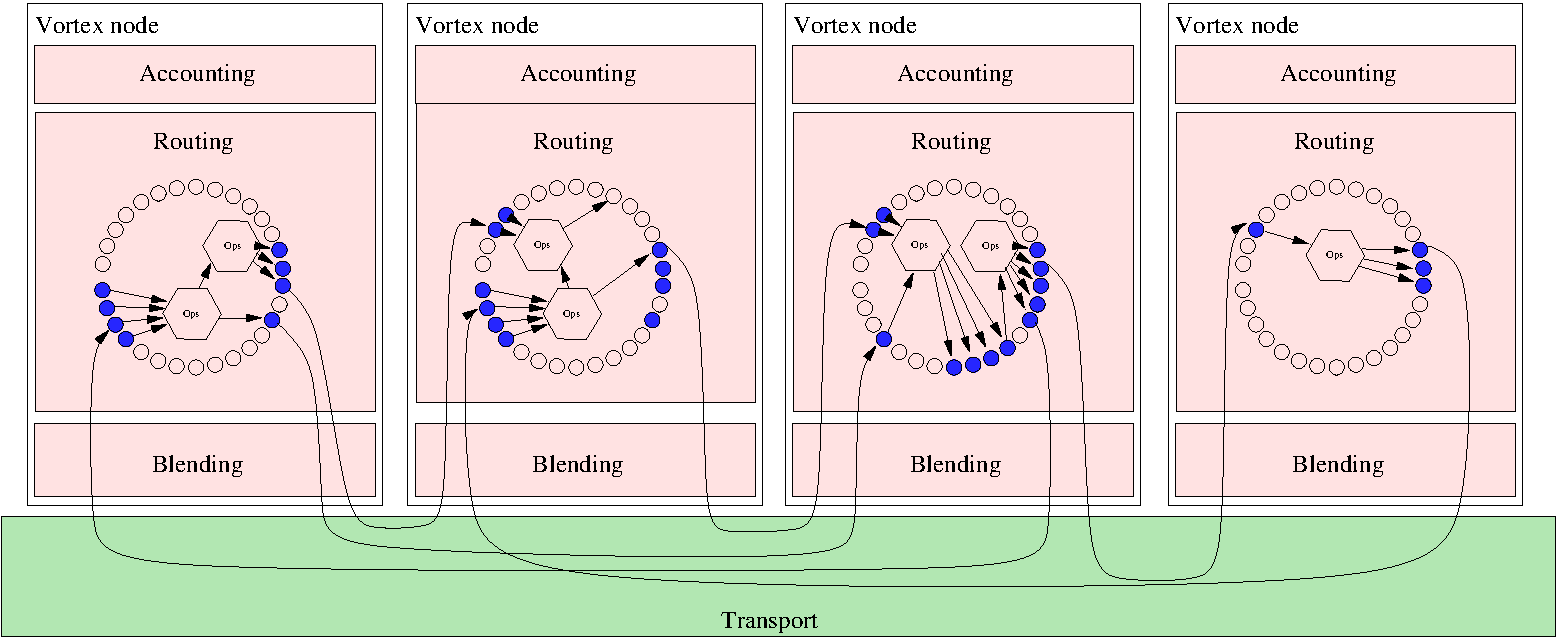
\includegraphics[width=2.5in]{../inc/roughProtocolDesign}
%\caption{Protocol stack.}
%\label{fig:layers}
%\end{figure}
The protocol is described precisely in \cite{MessageVortexRFC}. All necessary details to implement the protocol have been defi9ned in this document. 

We define the protocol on three different layers:
\begin{itemize}
	\item \emph{Blending layer:} in this layer, we embed vmessages into the transport protocol. 
	\item \emph{Routing layer:} this layer applies the logic to the message routing and prepares the message for the blending layer.
	\item \emph{Accounting layer:} this layer is a DoS and misuse protection. It keeps track of the transfers for each ephemeral identity and makes sure that queue and storage capacity are efficiently handled.     
\end{itemize}
These three layers are connected via the fourth layer. This layer is based on one or more store-and-forward based, common internet transport protocols. We refer to all protocols on this layer as transport protocols. It is important to note that no modification is applied to the transport protocol to accommodate vmessages.

All cryptographic operations such as encryption, decryption, hashing, or random number generation do not rely on a single algorithm. The protocol is able to signal what capabilities a node has and how exactly a message should be processed. This makes the protocol very robust if a used algorithm is broken. For this reason, we defined for each capability at least two algorithms which depend on different mathematical puzzles (e.g., ``integer factorization problem'' versus ``discrete logarithms problem''). This introduces redundancy in algorithms, allowing a sender to switch between algorithms if required.

\subsection{Protocol Layers}
\subsubsection{Transport}
The transport layer provides the Internet infrastructure. Unlike in most other approaches such as \cite{tor-design,sherwood2005p5,freenet}, this layer is not protocol specific. We use already existing, symmetrically built store and forward protocols. Attributes such as anonymity do not rely on the security of this layer.

By using this approach, we remove the need for shaky technologies such as TCP or UDP hole punching to connect peer partners. It furthermore makes the use of ``mostly connected'' clients such as mobile phones or DSL connections suitable for this protocol. This is because our transport endpoints are always reachable within the global network. The routing nodes may disconnect from time to time without affecting reachability of a mix. 

Protocols on this layer are typically well known and frequently used. They have no prerequisite for encryption or privacy and are store-and-forward based protocols with routing capabilities. 

\subsubsection{Blending}
This layer is a translation-only layer and embeds vmessages from the routing layer in transport protocol messages. Incoming vmessages are extracted from the transport layer and passed to the routing layer. Messages can be identified by picking a potential vmessage block up and start deciphering $k_{p_N}$ using its private key $k^{-1}_{h_N}$. If decryption succeeds, a vmessage block is found. This makes it impossible for an adversary to detect the presence of a vmessage without the hosts private key $k^{-1}_{h_N}$.

Protocol features such as anonymity or redundancy do not rely on this level. This layer embeds messages within the transport layer in such a way that an adversary is no longer able to identify vmessages from regular transport layer messages. Good blending is achieved if transport layer censorship measurements such as application-level firewalls are unable to detect the difference between real-world messages and vmessages. In an ideal application, this applies to human  and algorithmic censorship. 

In a real scenario, it is hard to achieve human proof censorship circumvention. If not done with care, problems, as described in \cite{abadi2005moderately}, arise. It is in our case not necessary as human censorship is very costly and slow compared to algorithms. Human censorship is too slow for real-time censorship. Our transport layer is by definition frequently used for regular communication. We always consider algorithm-based censorship as existing.

Currently, the specification of this layer is limited to the two capabilities ``embed with offset'' and ``F5''. 

``Embed with offset'' is a plain embedding of a block in a file attached to a message. The offset allows issuing first a valid header of some sort to improve blending (e.g., for a PCM-encoded WAV file). While this is considered very weak protection, analysis to detect such a file on a global transport scale is very demanding due to the sheer mass to be analyzed. 

``F5'' means applying the F5 algorithm to hide a message within a random suitable jpeg image. ``F5'' is one of the very few steganographic works which have a real-world implementation and attracted at least some interest in the research community. In \cite{steganalysisf5}, an approach to detect embedded information in steganographically modified images is presented. To obtain this information, a considerable effort in terms of calculation power is required. This makes it impractical for real-time censorship on our scale. It does, however, allow messages to be identified. Furthermore, It only discloses the fact that F5 is being used. It does not leak the content of a message, its immediate sender (apart from a socket), or message size.

\subsubsection{Routing}
The routing layer is the mixer of the system. It processes messages extracted by the blending layer and is supported by the accounting layer. Any related set of messages is processed by the routing layer by recombining payload with operations defined in section~\ref{sec:operations}. Due to the nature of these operations, a node is unable to tell whether the traffic flow processed is decoy traffic or an actual part of the message flow.

If a message is processed, a new vmessage is generated and passed on to the blending layer.

For a more precise working of the routing process see section~\ref{sec:processing}.

\subsubsection{Accounting}
The accounting layer protects a node from being overloaded or misused. Every sender must first apply for an ephemeral identity which is limited by lifetime. This is done by a proof-of-work algorithm. When an ephemeral identity is being created, the owner of the identity may route vmessages through a node. The ephemeral identity is assigned with message and size transfer quotas. Any identity may apply for a raise of quota as long as it is not expired. It is up to the node to decide whether a raise of quota is acceptable or not. If rejected, any sender might try to apply for a new ephemeral identity.

Due to the costs of maintaining multiple identities and their parental identities for anonymity of the original sender, the number of identities grows exponentially when growing a network of ephemeral identities. A sender might either introduce a new node to cut identity costs or maintain at higher identity costs a single node.

\subsection{Protocol Outline}
We define a protocol block which has an inner block structure as shown in Fig~\ref{fig:blocks}.

\begin{figure}[htb]
	\centering
	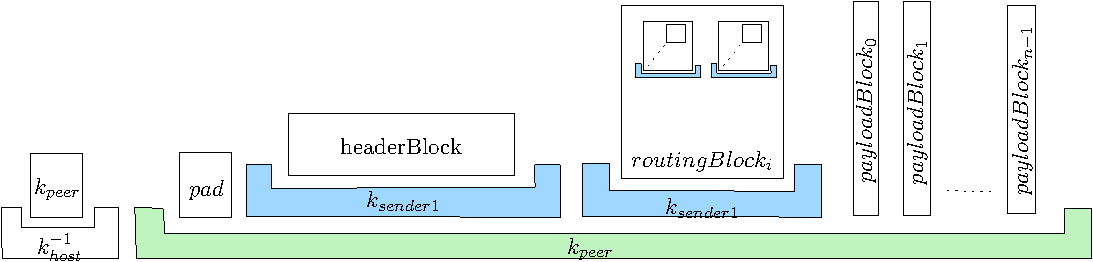
\includegraphics[width=\columnwidth]{../../inc/blockLayoutSimplified}
	\caption{Protocol block outline.}
	\label{fig:blocks}
\end{figure}

These blocks are passed from node to node. All blocks are binary proof, which means that the same block sent twice will always result in exactly the same bit layout. There is no room for a misbehaving node to tag the block within it without compromising the message. The message as a whole is replay protected. Routing and header blocks are linked with a chain secret to avoid hijacking of header or routing blocks.

\subsubsection{Message Keys}
Every protocol block is protected by two symmetric keys $key_{peer_N}$ (in short $k_{p_N}$) , $key_{sender_N}$ (in short $k_{s_N}$) and the private part of an asymmetric host key $k^{-1}_{host_N}$ (in short $k^{-1}_{h_N}$). The public host key $k^{1}_{h_N}$ and both symmetric keys are known to the builder of the routing block structure. 

This building is done by the sender. If using SURBs (Single-Use Reply Blocks), or MURBs (Multi-Use Reply Blocks) it is done by the builder of the reply block. 

The header is protected by the symmetric key $k_{s_N}$ and is found in a preamble to the header protected by the receiving peer's private key $k^{-1}_{h_N}$. The key $k_{s_N}$ is known to the routing block builder and the receiving node only. The receiving node obtains all important information protected by this key. $k_{p_N}$ is known to two immediate peers and the builder of the routing block. The sending peer obtains $k_{p_N}$ from the routing block, whereas the receiving peer acquires it in the $headerBlock$. 

\subsection{Pad Block}
The pad block is a short block of a few bytes of padding content (first bytes of the first message block; fixed size per message; null padded) guaranteeing that all messages sent with the same routing block look different on the transport layer.

\subsubsection{Header Block}
The header block contains vital static information for the message disclosed to only one peer of the network. It is protected by key $k_{s_N}$. The minimally contained information can be described by the list $headerBlock_i:=\langle sendingIdentity,\allowbreak{} serial_i,\allowbreak{} replayAttributes_i,\allowbreak{} key_{p_i},\allowbreak{} chainSecret,\allowbreak{} signature,\allowbreak{} optionalOperations \rangle$.

\subsubsection{Routing Block}
A routing block can be expressed with the following recursive definition $routingBlock_i:=\langle\allowbreak{} nexthopAddress,\allowbreak{} chainSecret,\allowbreak{} timingAttributes,\allowbreak{} E^{k_{s_{i+1}}}\left(headerBlock_{i+1}\right),\allowbreak{} E^{k_{s_{i+1}}}\left(routingBlock_{i+1}\right),\allowbreak{} payloadBuildInstructions_i,\allowbreak{} payloadId,\allowbreak{} optionalReplyBlocks \rangle$

\subsubsection{Payload Block}
A payload block is any number of bytes representing parts of a message, decoy traffic or a control block.

\subsection{Message Processing\label{sec:processing}}
Unlike with a traditional mix system, a node has no choice of sending. It purely relies on the message processing facilities. A message is either handed over to the transport layer by the blending layer or may be induced internally (if the local node is the sender). 

First, the preamble to the header is extracted. This proves that the sender possesses the public key of the node and contains the sender key $k_{s_i}$. With this information, the node opens the $headerBlock$ revealing information regarding the ephemeral identity of the original sender. Based on the information given in the relatively small header, the transport layer may decide whether further processing is desired or not. If desired, the node extracts the key $k_{p_i}$ and decrypts the rest of the message, which is considerably larger containing routing and payload information.

The routing block may contain instructions on processing information contained in this or any message related to this message and identity. These instructions are encoded in so-called ``Operations'' as specified in section~\ref{sec:operations} and may be any combination of them. As soon as the time arises for a routing block to be processed, the operations building the new message blocks are executed. If all prerequisites are satisfied, the new payload blocks are built, concatenated with the new routing block, pad, and header block. This resulting block is encrypted with $k_{p_{i+1}}$ and prepended with the preamble. The built block is passed to the blending layer with the blending specification and the target address.

It is important to note that the blending specification contains vital information about how the message must be blended but not how the carrier message looks like. By doing so, we avoid abuse of the blending layer (eg. sending plain text spam through the MessageVortex system).

\subsection{Operations\label{sec:operations}}
The operations are designed in such a way that they allow a variance of message size without telling anyone, including the generator, which message part is used later. They include features to protect message content from bugging.

Some of the operations require a pseudo-random number generator (PRNG). This PRNG is defined in Appendix~\ref{sec:prng}. The definition of a reproducible PRNG to be used by messages is important as we have to achieve binary proof messages.

All interactions are non-interactive. Interactive operations such as DC-nets do add more complexity to the system. Behavioral analysis can be used to identify interactive operations. 

This is one of the main reasons, why DC-nets are rarely used in this context. Theoretically, it is possible to reflect them as a single operation by calculating the answer and then broadcasting the answer. In practice, this fails due to the non-existence of efficient, reliable multicast networks. There are attempts to apply DC-nets to real protocols \cite{Corrigan-Gibbs:2010:DAA:1866307.1866346}.

\subsubsection{$\addRedundancy$ and $\removeRedundancy$ Operation}
This operation is based on a modified Reed-Solomon redundancy function to accommodate the anonymity needs of this function. The Reed-Solomon function as defined in Appendix~\ref{sec:reedSolomon} offers a varying number of redundant checksum blocks. When sending these blocks into multiple directions, no mixing node is able to tell where the original message is being rebuilt. The general inner workings are described in Fig~\ref{fig:addRedundancy}.

\begin{figure}[htb]
	\centering
	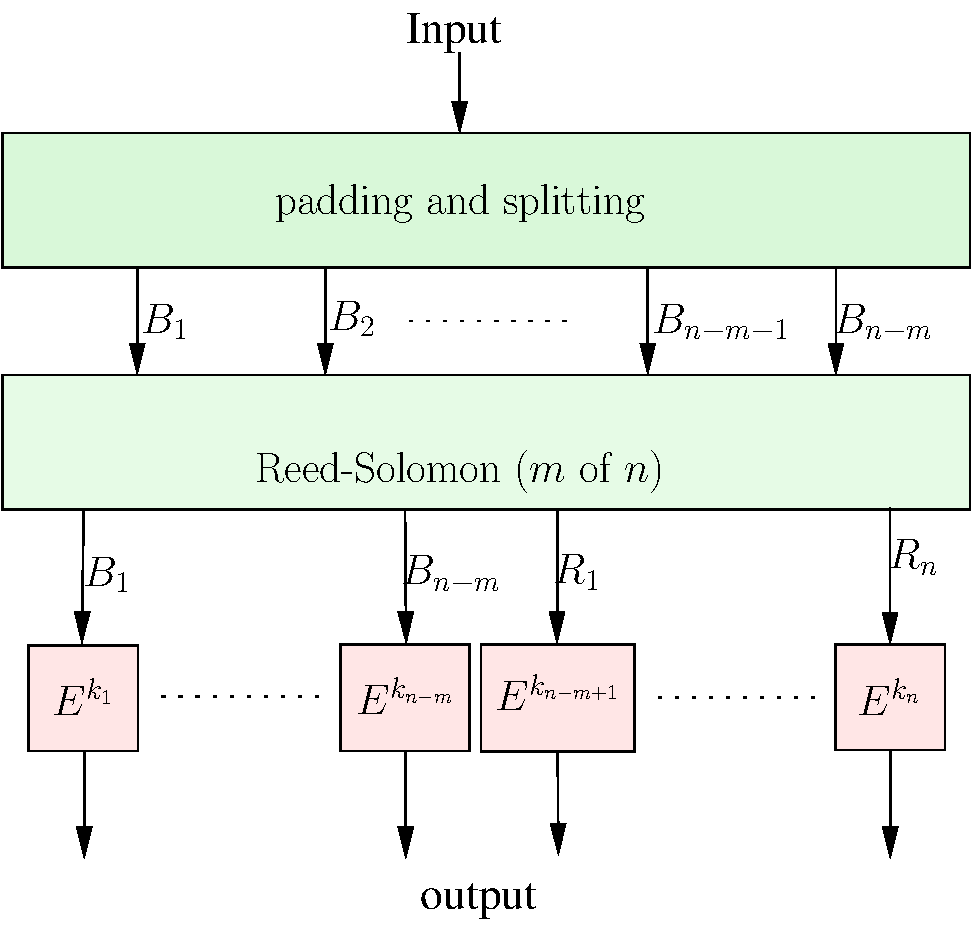
\includegraphics[width=2.5in]{../../inc/addRedundancyOp}
	\caption{AddRedundancy Operation}
	\label{fig:addRedundancy}
\end{figure}

We define a function $\addRedundancy_{n,m}( \mathbf{M},k_1\ldots k_{m} )$ where $M$ denotes the message, $n$ the number of total output blocks, $m$ the number of redundancy blocks whereas $m<n$, $k$ the encryption key and scheme to be used, and $bs_k$ the block size required to accommodate scheme and key size described by $k$. It is important to note that any set with the size of $d=n-m$ may be used to recover the full set of original data blocks.

By encrypting all output blocks individually, we make sure that no node having access to enough blocks may rebuild the data stream without the routing block builder's consent.

The message is length-prefixed with a big-endian 64 bit unsigned integer number and padded in such a way that $8+\len(M)+\len(padding) \bmod bs_k =0$. As padding stream, we take the output of $\prng_i\left(\left\lceil\frac{8+\len(M)}{b_s}\right\rceil b_s n\right )$. The first 64 bytes of the message (padded with 0 if required) are taken as initializer $i$ for the PRNG function. By preparing our message block in such a way, we guarantee that the output blocks are encryptable without further padding and that the output of all $addRedundancy$ functions is binary proof. If stream ciphers are used as output ciphers, then padding is not required.

The reverse function for $\addRedundancy$ is called $\removeRedundancy_{m,n}(B_1\ldots B_{m},k_1\ldots k_{m})=\mathbf{M}$ and recovers the original data stream if enough blocks (at least $m$) and respective valid keys are provided. 

\subsubsection{$\splitPayload$ and $\mergePayload$ Operation}
The $\splitPayload$ and $\mergePayload$ operations split and merge payload blocks ($pb_N$)into two chunks of different or equal sizes respectively joins them. We define the functions as follows:

If $\len(pb_1)$ expresses the size of a payload block called $pb_0$ in bytes then the two resulting blocks of the $splitPayload$ Operation $pb_1$ and $pb_2$ have to follow the following rules:

\begin{eqnarray}
\splitPayload(f, pb_0) & = &\langle pb_1, pb_2 \rangle\\
\startsWith(pb_0, pb_1)\\
\lendsWith(pb_0, pb_2)\\
\len(pb_2) & = & \left\lfloor \len(pb_0)\cdot f\right \rfloor\\
\len(pb_0) & = & \len(pb_1) + \len(pb_2)
\end{eqnarray}
respectively
\begin{eqnarray}
\mergePayload(pb_1, pb_2) & = & pb_0 \\
\startsWith(pb_0, pb_1)\\
\lendsWith(pb_0, pb_2)\\
\len(pb_0) & = & \len(pb_1) + \len(pb_2)
\end{eqnarray}

\subsubsection{$\encrypt$ and $\decrypt$ Operation}
$\encrypt$ and $\decrypt$ are used as message obfuscation operations. These operations may be applied if a block is passed on without any required operation. They minimise the risk for a known plain text attack to a MessageVortex block. Both operations are defined as a padded or unpadded symmetrical encryption. $spec$ is the encryption specification and key provided by the routing block.

The operations are defined as follows:
\begin{eqnarray}
\encrypt(pb_0) & = & pb_1 \\
\len(pb_1) & \geq & \len(pb_0)\\
\decrypt(pb_1) & = & pb_0
\end{eqnarray}

\subsection{Protocol Bootstrapping}
In order to allow bootstrapping of the protocol, any node may reveal a very small, fixed number of nodes known to it. This allows new nodes to bootstrap their knowledge about an existing network, given they know at least one node willing to reveal other nodes. 

Allowing this kind of bootstrapping has certain downsides. As no trust is given into the requester's identity, we have to be very careful here not to reveal the full network to any adversary. By applying the PoW and requiring an ephemeral identity, we assign a high cost to this operation. 

Another downside is that it takes a long time for such a network to balance its loads if a network increases over time in size. Mature nodes concentrate more traffic on them than younger ones. This does distribute more evenly over time if algorithms, as shown in \cite{messageVortex}, are applied.

\section{Results}
Our protocol may be seen as a toolset for creating and sending anonymized messages. The degree of anonymity and redundancy is created when building the routing block. This is why constraints on message building are important.

\subsection{Message Building}
\begin{figure}[htb]
	\centering
	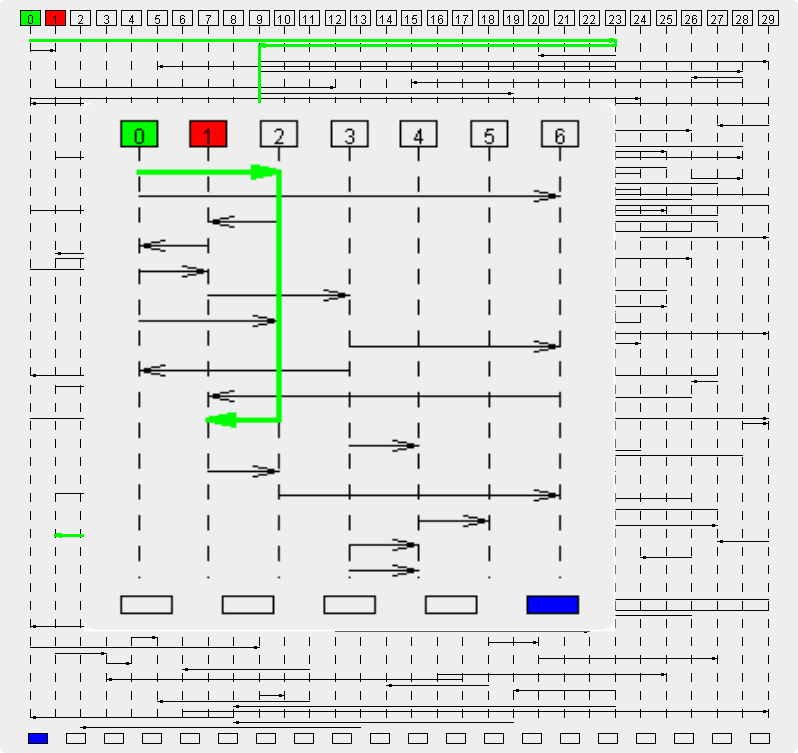
\includegraphics[width=0.8\columnwidth]{../msgGraph3}
	\caption{Message graphs with different numbers of nodes}
	\label{fig:mgsGraph}
\end{figure}

Using previously defined operations, we may build a message path. This path is typically built by first assigning an identity set $I_k$ where  $k$ denotes the target identity. $I_k$ is a static set of $n$ ephemeral identities $I_k\langle eI_1 \ldots eI_n\rangle$ which are always used to communicate with $k$. This set may be enriched with further $m$ ephemeral identities when sending. An identity set is replaced with a different one as soon as ephemeral identities expire. Therefore, we apply a new anonymity set unrelated to the old one with each new set of ephemeral identities.

A full message graph including all traffic may have any type of complexity. Fig~\ref{fig:mgsGraph} shows a graph with a $k$-Anonymity of $k=7$ of a message. It features five partially independent routes from source (edge 0) to the target (edge 1). One is highlighted in green. All involved nodes receive enough information to build the entire message if provided with the correct decoding instruction. The X-axis shows the involved nodes and the y-axis denotes the sequence in time. In its background, a graph with $k=30$ and 20 partially independent paths is shown.

When building the message, it has to be ensured that all nodes in $I_k$ obtain enough information to rebuild the message. If an adversary is able to identify the full message flow and knows all the operations applied to the message except for those on the entry and exit node, and at least a subset of $k=|I_{k_{uncompromised}}|$ where $k>1$ exists then we are still at $k$-Anonymity as an absolute worst case scenario. Thus, we can prove that attacks, as described in \cite{DanSer04}, are of very limited use. 

\subsection{Attacking the Message Flow}
In our thesis\cite{messageVortex} we analyze various kinds of attacks. Such as illicit behaving nodes, hijacking of header and routing blocks, analysis on payload blocks, traffic replay, analysis of infrastructure, and analysis on operations. Results have shown that the protocol is very resistant against most kinds of attacks.

We can  prove the effectiveness of replay protection even when assuming misbehaving nodes. Hijacking a routing block has very limited use. Prepending an own identity block to a hijacked routing block would break the message path. Thus, allowing an adversary to reveal all blocks built from this routing block out of the message traveling through the adversary node. He does not gain any information about other blocks. He may extract how much traffic is generated on the manipulated node out of these blocks. The real amount of traffic is, however, higher as some operations may have failed due to missing blocks.

We can easily show the effectiveness of the tagging and bugging protection. A misbehaving node has no room to tag a message without compromising the message's integrity. A tagged message will be discarded at the first non-misbehaving node.

\subsection{Routing Diagnosis}
If an interruption of a path is suspected, parts of the message may be obtained by the message block builder at any time. He may do this by either introducing fixed diagnostic paths into a routing block, which we refer to as implicit diagnosis, or he may send a second message picking up a block of the message at a node to be tested. We refer to this as explicit diagnostic.

Explicit diagnostics may be used as a kind of ``receipt'' from any node including but not limited to the terminal receiver of a message. Any block at any time of routing may be returned directly or indirectly to the original sender. The arrival of such a packet and content tells the sender at which point a message failed. If a diagnostic packet does not arrive, the routing block builder may build a diagnostic message picking up random packets on any suspected failing node.

% An example of a floating figure using the graphicx package.
% Note that \label must occur AFTER (or within) \caption.
% For figures, \caption should occur after the \includegraphics.
% Note that IEEEtran v1.7 and later has special internal code that
% is designed to preserve the operation of \label within \caption
% even when the captionsoff option is in effect. However, because
% of issues like this, it may be the safest practice to put all your
% \label just after \caption rather than within \caption{}.
%
% Reminder: the "draftcls" or "draftclsnofoot", not "draft", class
% option should be used if it is desired that the figures are to be
% displayed while in draft mode.
%
%\begin{figure}[!t]
%\centering
%\includegraphics[width=2.5in]{myfigure}
% where an .eps filename suffix will be assumed under latex, 
% and a .pdf suffix will be assumed for pdflatex; or what has been declared
% via \DeclareGraphicsExtensions.
%\caption{Simulation Results.}
%\label{fig_sim}
%\end{figure}

% Note that IEEE typically puts floats only at the top, even when this
% results in a large percentage of a column being occupied by floats.
% However, the Computer Society has been known to put floats at the bottom.


% An example of a double column floating figure using two subfigures.
% (The subfig.sty package must be loaded for this to work.)
% The subfigure \label commands are set within each subfloat command,
% and the \label for the overall figure must come after \caption.
% \hfil is used as a separator to get equal spacing.
% Watch out that the combined width of all the subfigures on a 
% line do not exceed the text width or a line break will occur.
%
%\begin{figure*}[!t]
%\centering
%\subfloat[Case I]{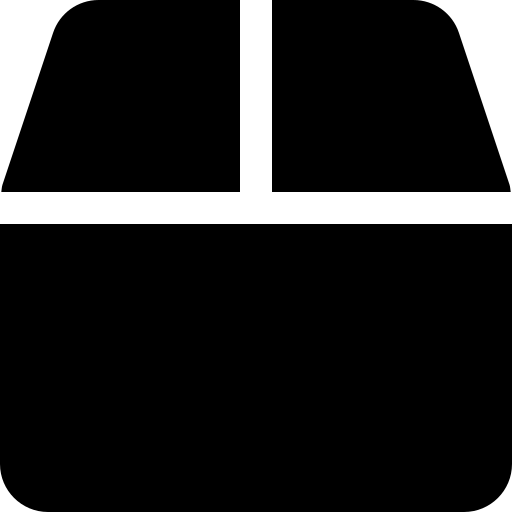
\includegraphics[width=2.5in]{box}%
%\label{fig_first_case}}
%\hfil
%\subfloat[Case II]{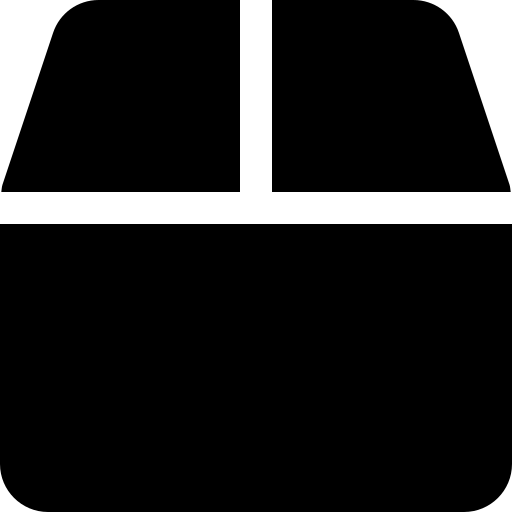
\includegraphics[width=2.5in]{box}%
%\label{fig_second_case}}
%\caption{Simulation results.}
%\label{fig_sim}
%\end{figure*}
%
% Note that often IEEE papers with subfigures do not employ subfigure
% captions (using the optional argument to \subfloat[]), but instead will
% reference/describe all of them (a), (b), etc., within the main caption.


% An example of a floating table. Note that, for IEEE style tables, the 
% \caption command should come BEFORE the table. Table text will default to
% \footnotesize as IEEE normally uses this smaller font for tables.
% The \label must come after \caption as always.
%
%\begin{table}[!t]
%% increase table row spacing, adjust to taste
%\renewcomma\cite{chaum-dc}\cite{chaum-dc}nd{\arraystretch}{1.3}
% if using array.sty, it might be a good idea to tweak the value of
% \extrarowheight as needed to properly center the text within the cells
%\caption{An Example of a Table}
%\label{table_example}
%\centering
%% Some packages, such as MDW tools, offer better commands for making tables
%% than the plain LaTeX2e tabular which is used here.
%\begin{tabular}{|c||c|}
%\hline
%One & Two\\
%\hline
%Three & Four\\
%\hline
%\end{tabular}
%\end{table}


% Note that IEEE does not put floats in the very first column - or typically
% anywhere on the first page for that matter. Also, in-text middle ("here")
% positioning is not used. Most IEEE journals use top floats exclusively.
% However, Computer Society journals sometimes do use bottom floats - bear
% this in mind when choosing appropriate optional arguments for the
% figure/table environments.
% Note that, LaTeX2e, unlike IEEE journals, places footnotes above bottom
% floats. This can be corrected via the \fnbelowfloat command of the
% stfloats package.

\section{Discussion}

\subsection{Comparison to Existing Systems}
The following section gives a short comparison to existing systems. It shows that the solution defined in this paper covers a different approach and what problems are solved. It is important to note that this is not a ranking. It just outlines the differences between the system and shows where our system is different compared to existing solutions.

\subsubsection{TOR}
%TOR has attracted considerable efforts from the scientific community in both attacking and defence. As an immediate result numerous attacks and counter measures exist within TOR. It was however never designed to withstand such a harsh definition for an adversary as we used it. TOR fails therefore in several aspects. Numerous attacks as outlined previously will succeed when assuming our adversary. 
%
TOR is criticised for several things. Firstly, it is easy attackable if encryption is not used in the transported protocol. It relies on the trust in a centralized directory infrastructure. It is susceptible if more than $\approx 30\%$ of the nodes are controlled by an adversary as shown in \cite{jansen2014sniper}. Furthermore, timing analysis on entry and exit nodes are particularly easy due to the fact that TOR is a low latency network\cite{torta05,esorics10-bandwidth}. Harvesting of nodes is possible (e.g., \url{https://torstatus.blutmagie.de}). Tor nodes are easily identifiable by traffic as shown in \cite{foci12-winter}. To avoid this detection TOR uses ``pluggable transports.'' Unlike in MessageVortex, this is not used in general but only when specifically set up between two nodes.

MessageVortex tries to address these problems in multiple ways. First, there is no central infrastructure which defies the trust problem. There are no entry or exit nodes as all participating members are routers at the same time. Therefore, all problems related to entry and exit nodes do not exist. There is no dedicated transport protocol making the presence of vmessages hard to detect.

MessageVortex has several downsides compared to TOR. It is not suitable for real-time communication due to its asynchronous operation. It is furthermore a closed system and only participating members may use it. %In contrast, TOR allows to tunnel almost any traffic through it to any destination. 

\subsubsection{$\mathcal{P}^5$}
%The Peer-to-Peer Personal Privacy Protocol is defined in \cite{sherwood2005p5}. It provides sender-, receiver- and sender-receiver anonymity. According to the project page of $\mathcal{P}^5$ there is only a simulator available for the protocol.
%
%The transport layer issue has been completely ignored. 
In-depth analysis of $\mathcal{P}^5$ is very limited, as there is no precise protocol specification but only a rough outline available. This outline specifies the messaging and the crypto operations only. It claims to be peer to peer, which would result in some kind of NAT (Network Address Translation) circumvention technology. This technology usually relies, at least partially, on a central infrastructure (e.g., for hole punching). 

In contrast, MessageVortex protocol is peer to peer, but the transport layer is not. It misuses already existing infrastructure for transport. This makes it not susceptible to approaches against infrastructure unless our messages are identified and filtered. This may be corrected by applying different blending schemes for the transport layer. It furthermore removes the need for NAT hole punching and similar technologies.

\subsubsection{$I^2P$}
%The name $I^2P$ is derived from  ``Invisible Internet Project'' according to \href{https://geti2p.net/}{geti2p.net}. The system itself is comparable to TOR in its capabilities. Mayor differences are:
%\begin{itemize}
%	\item P2P based
%	\item Packet switched routing (TOR is ``circuit switched'')
%	\item Different forward and backward routes (called tunnels)
%	\item Works pseudonymously
%	\item Supports TCP and UDP
%\end{itemize}
%
$I^2P$ has not attracted as much attention as TOR so far. It is thus hard to judge its real qualities. 

Unlike TOR, anonymity is not fully granted. Instead, pseudonymity is used. 

In \cite{pets2011-i2p} an attack specific to $I^2P$ is presented. As $I^2P$s security model is chosen based on IP addresses, the authors propose to use several cloud providers in different B-Class networks. By selectively flooding peers, an adversary may extract statistical information. The paper proposes an attack based on the heuristic performance-based peer selection. The main criticism of the paper was that the peer selection might be influenced by an adversary enabling him to recover data on a statistical base.

MessageVortex does only allow a routing block builder to choose routes and amount of traffic. Due to the replay protection and the trust model, we do not rely on any node. We show in \cite{messageVortex} that attacks on this level are ineffective.

\subsubsection{Freenet}
%Freenet was originally designed to be a fully distributed data store\cite{freenet}. Documents are stored in an encrypted form. Downloaders must know a document descriptor called CHK containing the file hash, the key, and some background about the crypto being used. A file is stored more or less redundantly based on the number of accesses to a stored file. The main goal of Freenet is to decouple  authorship from a particular document. It furthermore provides a fault tolerant storage, which improves caching of a document if requested more often.
%
While Freenet is a purely distributed storage system it has many good features adapted by MessageVortex. Like in Freenet a MessageVortex node may deny being the owner of specific information unless the key for the respective ephemeral identity can be found on the system. As the key is only required for building routing blocks but not for message assembly and sending, this makes it a valuable feature comparable to the deniability of Freenet.

\section{Conclusion}
The MessageVortex protocol outlined in the previous sections does not solve all privacy issues which might arise. Furthermore, it is complicated to implement and involves a considerable amount of bookkeeping at runtime which is left to the sender of a message and the mixing nodes. 

On the positive side, we have a new protocol which addresses privacy in a holistic approach leaving very little attack surface. If handled with appropriate care by the sender and receiver, the protocol allows a sender-controlled, high degree amount of anonymity. Message paths are diagnosable, may be built redundant and do not build on the trust of any third party systems including all involved mixes except the sender's and receiver's one. Even closed group communication or broadcasting to multiple identities involving a specific subset of mixes is possible if desired by the sender.

In \cite{messageVortex} we show that the protocol is very secure. It is hard to block as messages may be redundant, hard to identify as messages are covered within message flows which may not be blocked without a huge impact on existing systems. It is hard to apply censorship in a real-world scenario as messages are extremely hard to detect. 

MessageVortex has some flaws which must be outlined. We always considered algorithmic censorship. If human censorship is applied, we must assume that at least some of the messages are being identified as potential MessageVortex messages. If we assume a white-listing, human, censoring adversary (everything which is not identified by a human as compliant is censored) we must conclude that at least some messages will fail to be delivered. 

Some of the participating transport nodes may be identified and blocked. This may be compensated with redundancy in message transmission. 

Messages transported by MessageVortex generate huge amounts of decoy traffic. Unlike other systems which control decoy traffic on a ``per peer'' base, MessageVortex does not dynamically reduce decoy traffic as decoy traffic is not identifiable. This results in a huge traffic overhead.


% if have a single appendix:
%\appendix[Proof of the Zonklar Equations]
% or
%\appendix  % for no appendix heading
% do not use \section anymore after \appendix, only \section*
% is possibly needed

% use appendices with more than one appendix
% then use \section to start each appendix
% you must declare a \section before using any
% \subsection or using \label (\appendices by itself
% starts a section numbered zero.)
%

\newpage
\appendix

\section{Reed-Solomon Function\label{sec:reedSolomon}}
The origins of the Reed-Solomon code go back to \cite{reed1960polynomial}. The method described in this paper was however not applicable in all cases. The publications \cite{karnin1983secret} and \cite{Rabin:1989:EDI:62044.62050} describe a more practical solution whereas \cite{preparata1989holographic} brings up the similarity to the Reed-Solomon code with a $GF(2^\omega)$. 

Reed-Solomon is used for many applications today. One of the most well-known application is a redundancy generator for RAID-6 like systems. It is able to generate multiple linearly independent equation systems to a given set of data $B_1\ldots B_{n-m}$ creating redundancy information $R_1\ldots R_m$. In a system with all blocks $\langle B_1\ldots B_{n-m}, R_1\ldots R_m \rangle$ any number $k$ where $0\le k\le m$ data blocks may be removed and the information contained in $\langle B_1\ldots B_{n-m}\rangle$ is still recoverable. 

Traditionally the data and redundancy information is stripped into blocks and distributed together with the redundancy information overall $n$ storages. This is done to avoid data storages as bottleneck since a change to one data stripe  in a stripe set results always in a change of the redundancy data on the other $m$ redundancy storages. This would result in hot spots on redundancy information storages.

We use the Reed-Solomon function as redundancy generating function shown in Fig~\ref{fig:addRedundancy}. Unlike in storage technology, we encrypt each redundancy block and all data stripes individually. By doing so, we make it impossible to recover the contained information without knowledge of the keys. All blocks do then contain the same amount of data. Given we have enough blocks and the corresponding keys we may rebuild the message. 

At the same time, the generating node is unable to tell what blocks belong to the true message path and what blocks are sent for decoy traffic only. 

As our resulting blocks are encrypted with a stream or block cipher, we need to introduce some padding. The padding is applied before doing RS calculation. In the case of a stream cipher, we need to pad so that the number of bytes is dividable by the number of data blocks. In the case of block ciphers we need to pad so that all resulting data blocks have exactly a size dividable by the block size. We achieve two goals by applying the padding before splitting the blocks. First, we reduce overhead by adding only one instead of $n$ paddings. Secondly, an unpadded block is much harder to brute force. Any resulting block to a key might be the right one as we no longer have padding to suggest that decryption has been successful.

We defined to use Vandermonde matrices as outlined in \cite{pd:96:rs} and in \cite{pd:03:rs} for our redundancy calculations. For more information on the used GF-Fields and on exact matrix building instructions see \cite{messageVortex}.

\section{Adversary Model\label{sec:adversary}}
We assume as an adversary a state-sponsored actor who has unlimited monitoring possibilities on the network layer within a limited geographic region (e.g., country). We furthermore assume available funding and capabilities to efficiently run a considerable number of nodes (not exceeding the number of $70\%$) within the network and harvest and combine all operations and content processed by these nodes.

This means he is at least capable of analyzing traffic by algorithms and may disrupt any unwanted traffic.

The adversary is capable of generating any traffic anywhere within the message flow.

This is an adversary model which goes far beyond any model we have encountered in any other scientific approach.

Assumptions in this part are mostly derived from \cite{foci12-winter} and extrapolated. In this paper, researchers describe GFC (Great Firewall of China) as a profiling firewall fingerprinting traffic and blocking specific socket addresses when positively identified as TOR nodes. 

\subsection{Detection\label{sec:detCons}}
Any adversary may use detection schemes to detect traffic. This may be used to apply censorship later. He is capable of analyzing up to $1\%$ of the total transfer volume on an in-depth algorithmic base and $50\%$  based on simple context-less rules. 

\subsection{Censorship}
We assume that an adversary is accepting considerable economic damage but not the downfall of its own economy as a whole. An active adversary may apply algorithmic censorship based on the detection constraint (\ref{sec:detCons}) on a large scale.

\subsection{Information Retrieval}
We assume an adversary to be interested in all sorts of information available around messages. We consider the triple ``sender,'' ``receiver,'' and ``content'' as the most valuable set of information for an adversary. Other important pieces of information are:

\begin{itemize}
	\item The frequency of message interchange
	\item The message size
\end{itemize}

For the system we consider the following information as interesting for an adversary (descending order):
\begin{itemize}
	\item Routing nodes
	\item Transporting nodes
	\item Routing operations
	\item Routing (ephemeral) identities
	\item Routing volumes
\end{itemize}


% you can choose not to have a title for an appendix
% if you want by leaving the argument blank

% use section* for acknowledgement
\section*{Acknowledgments}
The authors would like to thank their families for being so patient with them, and all the people who took the time to review the paper, criticising it, and their questions outlining the papers weaknesses.
%
% ---- Bibliography ----
%
% BibTeX users should specify bibliography style 'splncs04'.
% References will then be sorted and formatted in the correct style.
%
\bibliographystyle{splncs04}
% \bibliography{mybibliography}
\bibliography{../../inc/bib/unclassified/Anonbib/anonbib,../../messagevortex}

%
%\begin{thebibliography}{8}
%\end{thebibliography}
\end{document}
